\documentclass[12pt, twoside]{article}
\usepackage[francais]{babel}
\usepackage[T1]{fontenc}
\usepackage[latin1]{inputenc}
\usepackage[left=7mm, right=7mm, top=7mm, bottom=7mm]{geometry}
\usepackage{float}
\usepackage{graphicx}
\usepackage{array}
\usepackage{multirow}
\usepackage{amsmath,amssymb,mathrsfs}
\usepackage{soul}
\usepackage{textcomp}
\usepackage{eurosym}
 \usepackage{variations}
\usepackage{tabvar}


\pagestyle{empty}

\begin{document}

\begin{center}
\textbf{Correction devoir surveill� 2}
\end{center}

\bigskip


\ul{Exercice 5}
 



\begin{center}
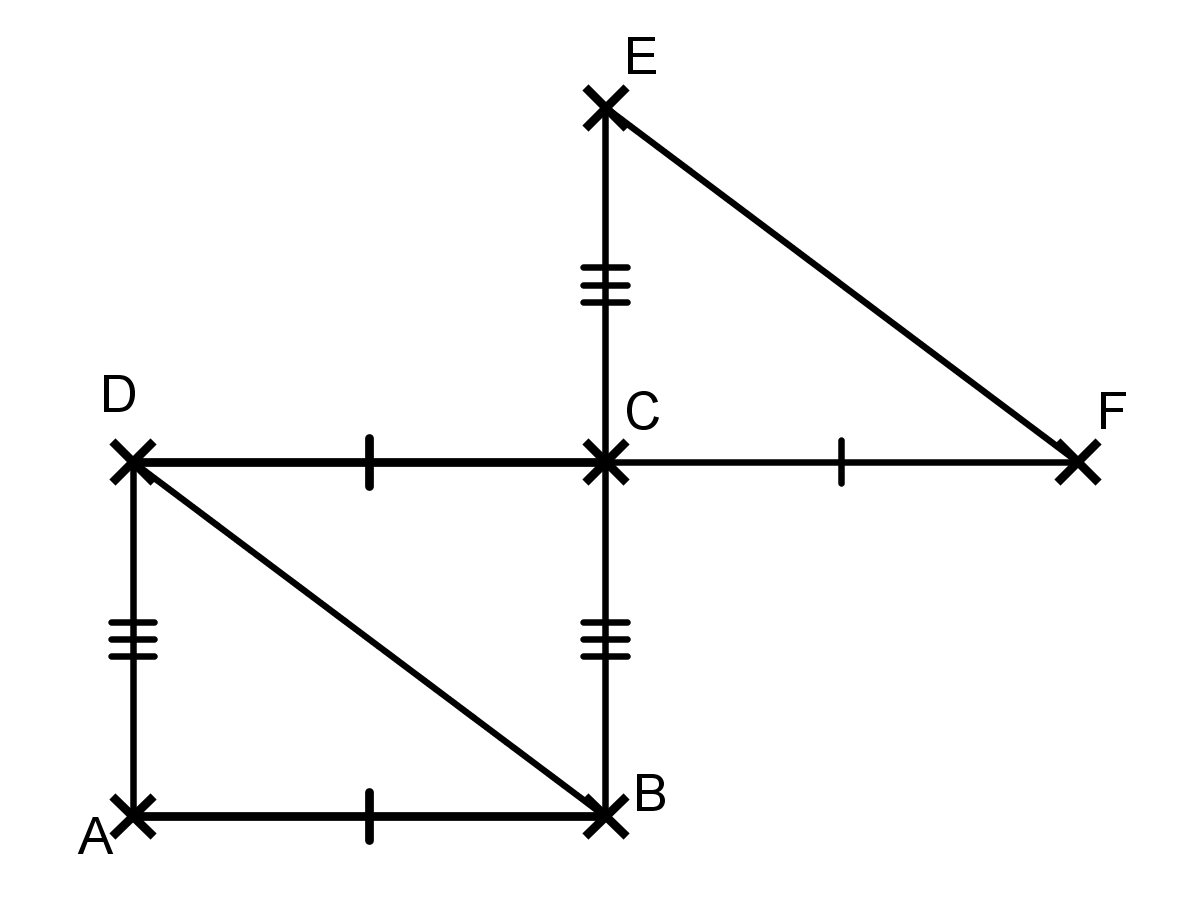
\includegraphics[width=5cm]{images/ex5.png}

\end{center}


\begin{enumerate}
  \item [4)] BC=CE donc \ldots \ldots et \ldots \ldots sont sym�triques par
  rapport � \ldots \ldots. 

  C est son propre sym�trique par rapport au point C.  

  DC=CF donc \ldots \ldots et \ldots \ldots sont sym�triques par
  rapport � \ldots \ldots.  
  
  
  Donc les triangles \ldots \ldots et \ldots \ldots sont sym�triques par
  rapport � C.
  \item [5)] D et \ldots \ldots sont sym�triques par rapport � C. 
  
  B et \ldots \ldots sont sym�triques par rapport � C.
  
  Donc les segments  \ldots \ldots et \ldots \ldots sont sym�triques par
  rapport � C. Deux segments sym�triques ont m�me \ldots \ldots \ldots \ldots,
  on en d�duit: DB= \ldots.
  \item [6)] D et \ldots \ldots sont sym�triques par rapport � C. 
  
  B et \ldots \ldots sont sym�triques par rapport � C. 
  
  Donc les droites \ldots \ldots et \ldots \ldots sont sym�triques par rapport
  � C. Deux droites sym�triques par rapport � un point sont \ldots \ldots
  \ldots \ldots donc: 
\end{enumerate}

\bigskip


\begin{center}
\textbf{Correction devoir surveill� 2}
\end{center}

\bigskip


\ul{Exercice 5}
 



\begin{center}
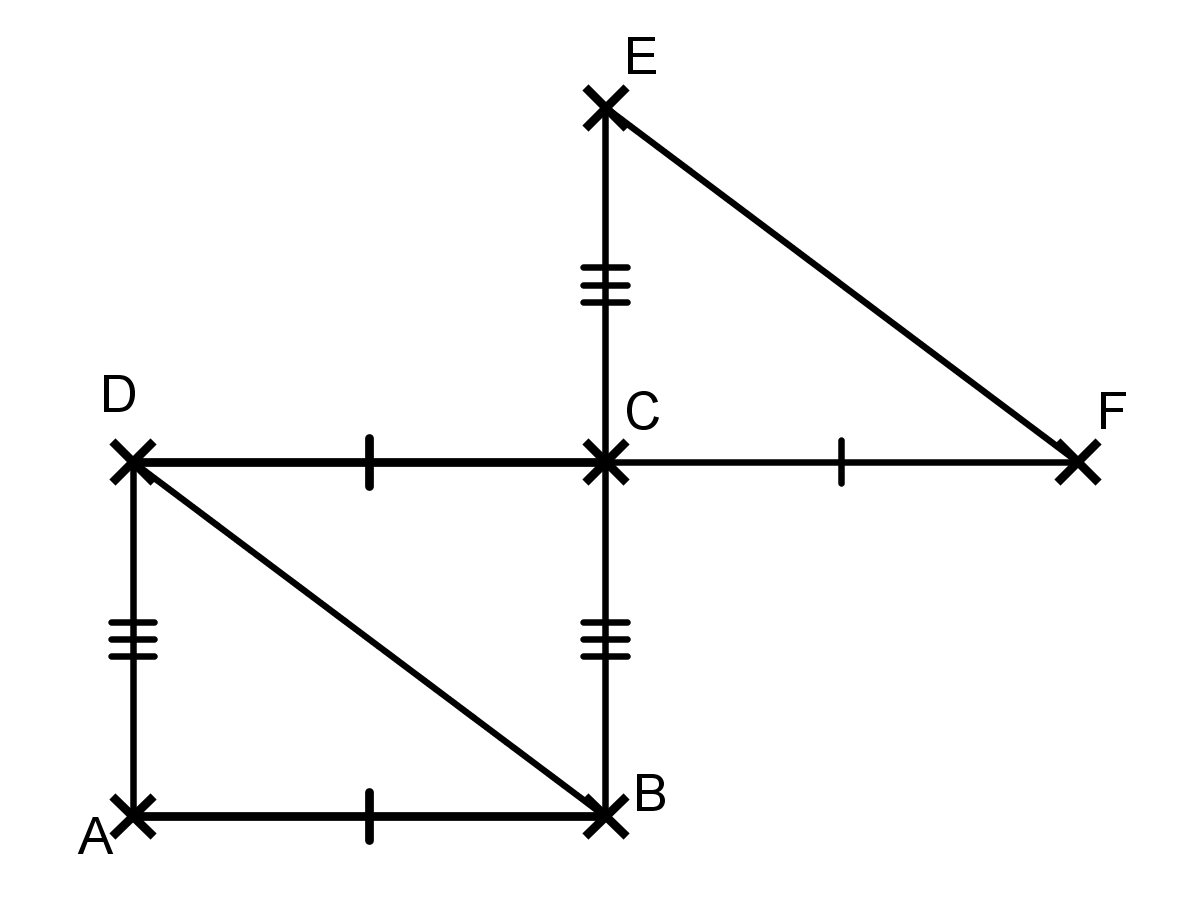
\includegraphics[width=5cm]{images/ex5.png}

\end{center}


\begin{enumerate}
  \item [4)] BC=CE donc \ldots \ldots et \ldots \ldots sont sym�triques par
  rapport � \ldots \ldots. 

  C est son propre sym�trique par rapport au point C.  

  DC=CF donc \ldots \ldots et \ldots \ldots sont sym�triques par
  rapport � \ldots \ldots.  
  
  
  Donc les triangles \ldots \ldots et \ldots \ldots sont sym�triques par
  rapport � C.
  \item [5)] D et \ldots \ldots sont sym�triques par rapport � C. 
  
  B et \ldots \ldots sont sym�triques par rapport � C.
  
  Donc les segments  \ldots \ldots et \ldots \ldots sont sym�triques par
  rapport � C. Deux segments sym�triques ont m�me \ldots \ldots \ldots \ldots,
  on en d�duit: DB= \ldots.
  \item [6)] D et \ldots \ldots sont sym�triques par rapport � C. 
  
  B et \ldots \ldots sont sym�triques par rapport � C. 
  
  Donc les droites \ldots \ldots et \ldots \ldots sont sym�triques par rapport
  � C. Deux droites sym�triques par rapport � un point sont \ldots \ldots
  \ldots \ldots donc: 
\end{enumerate}
\end{document}
